\documentclass[12pt]{article}
\usepackage{graphpap}
\usepackage[dvipsnames]{xcolor}
%\usepackage[10pt]{moresize}
%\usepackage[utf8]{inputenc}
\usepackage{latexsym,amsfonts,amssymb,amsthm,amsmath}
\usepackage[letterpaper, portrait, margin=0.7in]{geometry}
\usepackage{parskip}
\usepackage{tkz-euclide}
\usepackage{pgfplots}
%\usepackage{newtxtext}
\graphicspath{{\string~/Desktop/UW/1B/MATH148/MATH-148-Notes}}
\usepackage{hyperref}
\hypersetup{
    colorlinks=true,
    linktoc=all, 
    linkcolor=black,}


\usetkzobj{all}

%\usepackage{stix}

\theoremstyle{plain}

\newtheorem{theorem*}{Theorem}[subsection]
\newtheorem{theorem}{Theorem}[subsection]
\newtheorem{thm}{\textit{Theorem}}[subsection]
\newtheorem{definition}{Definition}[subsection]
\newtheorem{lemma}{Lemma}[subsection]
\newtheorem{conjecture}{Conjecture}[subsection]
\newtheorem{proposition}{Proposition}[subsection]
\newtheorem{example}{Example}[subsection]
\newtheorem{corollary}{Corollary}[subsection]
\newtheorem{algorithm}{Algorithm}[subsection]
\newtheorem{notation}{Notation}[subsection]


%      Blackboard bold letters
%\newcommand {⟨cmd⟩} [⟨num⟩] [⟨default⟩] {⟨definition⟩}
\newcommand{\abs}[1]{\left| #1 \right|}
\newcommand{\mC}{{\mathbb{C}}}
\newcommand{\mN}{{\mathbb{N}}}
\newcommand{\mQ}{{\mathbb{Q}}}
\newcommand{\mR}{{\mathbb{R}}}
\newcommand{\mZ}{{\mathbb{Z}}}
\newcommand{\Mod}[1]{\ (\mathrm{mod}\ #1)}
\newcommand{\de}{\delta}
\newcommand{\ep}{\varepsilon}
\renewcommand{\phi}{\varphi}
\newcommand{\dlim}{\displaystyle\lim\limits}
\newcommand{\dsum}{\displaystyle\sum\limits}
\let\emptyset\varnothing

\DeclareMathOperator{\Dom}{dom}
\DeclareMathOperator{\Img}{img}
\DeclareMathOperator{\Par}{partition}

\begin{document}
	\begin{titlepage}
	\begin{center}
		\textbf{\large Math 148  Notes}\\[1ex]
		\large{velo.x}\\ 
	\end{center}
	\vfill
	Instructor: Nico Sprunk \\
	Section: 002
	\end{titlepage}
	\newpage
	

\tableofcontents\label{toc}


\newpage

\section{INTEGRATION}
	MOTIVATION: area, let $a<b$ in $\mathbb{R}$, and 
	let $f:[a,b]\to [0,\infty]$, let 
	\[
		S_f = \{(x,y): 0\leq y\leq f(x), x\in [a,b]\} ("subgraph")
	\]
	IDEA: area of rectangel = height * width

	\begin{enumerate}
		\item 
			$ $
		 \begin{figure}[htbp]
    	\centering
    	\caption{The area under the function $\frac1x$ is $\log x$}
    	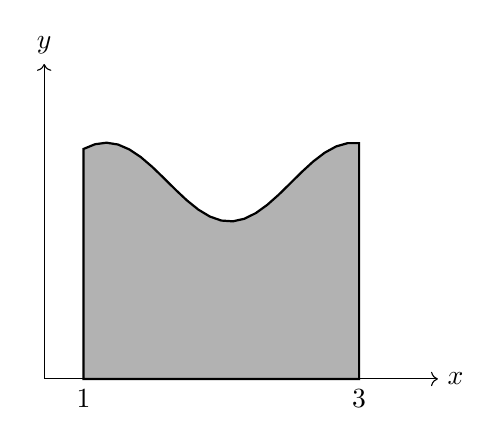
\begin{tikzpicture}[scale=0.5]
    		\draw[->] (0,0) -- (0,8) node[above] {$y$};
    		\draw[->] (0,0) -- (10,0) node[right] {$x$};

    		\filldraw[black!30,domain=1:8,variable=\x,draw=black,thick]
					(1,0) node[below,black,opacity=1] {$1$}
					-- plot (\x,{sin(\x r)+5})
					-- (8,0) node[below,black,opacity=1] {$3$}
					-- cycle;
			\end{tikzpicture}
		\end{figure}


			
	
		\item approximate $S_f$ by rectangle from below 13:43 JAN 6, 
			
			$j = 1, \cdots, 4$, $m_j = \inf\{f(x): x\in [x_{j-1}, x_j]\}$
			\[
				\sum_{j=1}^4 m_{j-1} (x_i-x_{j-1})\leq area(s_f)
			\]
		\item approximate $S_f$ by rectangle from above,
			$M_j = \sup\{f(x) : x\in [x_{j-1},x_j]\}$
			\[
				area \leq \sum_{j=1}^4 M_j (x_j - x_{j-1})
			\]
		\item if we can arrange lower sum $\approx$ upper sum, then we have 
			some good approximation
	\end{enumerate}

	\vspace{0.3 in}



	\subsection{Partition, Upper and Lower Sum}
	Let $a<b \in \mathbb{R}$, $f:[a,b]\in\mathbb{R}$,

	\begin{definition}[\textbf{Partition}]
		A \textbf{partition} of $[a,b]$ is any finite set of points including
		the endpoints. 
		\[
			P:\{x_0,x_1,\cdots, x_n\} s.t. a=x_0<x_1<\cdots<x_n=b
		\]
		often for convenience, we write $P=\{a=x_0<\cdots<x_n=b\}$.
	
		A \textbf{Refinement} of $P$ is any partition $Q$ of $[a,b]$ s,t,
		$P\subseteq Q$.\\
	\end{definition}
	
	Now, fix a partition $P$ of $[a,b]$ and let $f:[a,b]\to \mathbb{R}$ be 
	bounded on $[a,b]$, i.e. $\underset{x\in [a,b]}{sup} 
	\abs{f(x)}\leq M<\infty$.	
	Write $P=\{a=x_0<\cdots<x_n=b\}$. For $j = l, \cdots, n$, 
	\begin{align*}
		m_j &= m_j(P) = \inf \{f(x) : x\in [x_{j-1},x_j]\}\\
		M_j &= M_j(P) = \sup \{f(x) : x\in [x_{j-1},x_j]\}
	\end{align*}
	Notice that $-M\leq m_k\leq M_j\leq M$ for each $j$, and these "inf", "sup"
	exist. (Using that $\mathbb{R}$ is complete.)\\

	We then define after Riemann-Darboux for $P$ and $f$ as above. 

	\begin{definition}
		$ $
		\begin{itemize}
			\item \textbf{Lower Sum:} $L(f, P) = \sum_{j=1}^n m_j 
				\underbrace{(x_j-x_{j-1})}_{width\ of\ [x_{j-1},x_j]}$
			\item \textbf{Upper Sum:} $U(f, P) = \sum_{j=1}^n M_j 
										(x_j-x_{j-1})$
		\end{itemize}
	\end{definition}

	\textbf{Remark: }
	\begin{enumerate}
		\item if $f$ is not bounded, at least one of $L:(f,P)$ or $U(f, P)$ 
			cannot be defined. 
		\item we have $L(f, P)\leq U(f,P)$, Indeed, for each $j=l,\cdots, n$,
			$m_j\leq M_j$. (exactly from definition), 
			\[
				L(f, P) = \sum_{j=1}^n m_j (x_j-x_{j-1})\leq
				\sum_{j=1}^n M_j (x_j-x_{j-1}) = U(f, P)
			\]
	\end{enumerate}

	\begin{lemma}
		If $P$ is a partition of $[a,b]$, $f:[a,b]\to \mathbb{R}$ is bounded,
		and $Q$ is a refinement of $P$, then 
		\[
			L(f,P)\leq L(f,Q) \qquad U(f,Q) \leq U(f,P)
		\]
	\end{lemma}
	\begin{proof}
		$ $\\
	\begin{itemize}
		\item Case 0: $Q = P$ obvious

		\item Case 1: $Q = P \cup \{q\}$ where $q\not\in P$, 

		write $ P = \{a = x_0<\cdots,x_n=b\}$ so 
		$Q = \{a=x_0<\cdots<x_{k-1}<q<x_k<\cdots<x_n=b\}$
		Then, 
		\begin{align*}
			m_k(P) &=\inf \{f(x):x\in[x_{k-1}],x_k\} 
			\qquad [x_{k-1},x_k] = [x_{k-1},q]\cup [q,x_k] \\
			&= \min\{\inf\{f(x): x\in [x_{k-1}, q]:x\in [x_{k-1},q]\}
			\inf f(x):x\in [q,x_k]\}\\
			&=\min\{m_k(Q), m_k'(Q)\} \leq m_k(Q), m_k'(Q)
		\end{align*}
		Thus, 
		\begin{align*}
			L(f,P) &=\sum_{j=1}^m m_j(P)(x_j-x_{j-1}) \\
				   &=\sum_{j=1}^{k-1} m_j(P)(x_j-x_{j-1})+m_k(P)(x_k-x_{k-1})
				   +\sum_{j=k+1}^n m_j(P)(x_j-x_{j-1}) \\
				   &\leq \sum_{j=1}^{k-1} m_j(P)(x_j-x_{j-1})+m_k
		\end{align*}
		
		\item Case 2: $Q = P\cup\{q_1, \cdots, q_m\}, q_1,\cdots,q_m$ distinct, 
		$q_u\not\in P$, by case 1, we have
		\[
			L(f,P) \leq L(f, P\cup\{q_1\})\leq L(f,P\cup\{q_1,q_2\})\leq \cdots
			\leq L(f,P\cup\{q_1,\cdots,q_m\}) = L(f,Q)
		\]
		The case $U(f,Q)\leq U(f,P)$ is similar. 
		\end{itemize}
	\end{proof}



	\begin{corollary}
		let $P, Q$ be any partition of $[a,b]$ and $f:[a,b]\to \mathbb{R}$ be 
		bounded, then 
		\[
			L(f,P)\leq U(f,Q)
		\]
	\end{corollary}
	\begin{proof}
		We have $P,Q \subseteq P\cup Q$, i.e. $P\cup Q$ refines each of $P$ and
		$Q$.
		Thus, 
		\[
			L(f,P)\leq L(f,P\cup Q) \leq U(f,P\cup Q) \leq U(f,Q) 
		\]
		
	\end{proof}







	\subsection{Integral and Upper and Lower Sum}

	\begin{definition}
		Given a bounded $f:[a,b]\to\mathbb{R}$, define 
		\begin{itemize}
			\item \underline{lower integral} : 
				$\underline{\int} 
				a^b f = \sup \{L(f,P): P \ is\ a\ partition \ of \ [a,b]\}$
			\item \underline{Upper Integral:}
				$\bar{\int}_a^b f = \inf \{U(f,Q): Q\ is \ a \ partition
				\ of \ [a,b]\}$
		\end{itemize}
		\textbf{Note}:
		$\underline{\int}_a^b f
		=\sup \{L(f,P): P \ is\ a\ partition \ of \ [a,b]\}
		\leq \inf \{U(f,Q): Q\ is \ a \ partition \ of \ [a,b]\} 
		=\bar{\int}_a^b f$
	
		We say that $f$ is \textbf{integrable} on $[a,b]$ provided that 
		\[
			\underline{\int}_a^b f = \bar{\int}_a^b f
		\]
		In this case, we write $\int _a^b f =  \bar{\int}_a^b f
		=\underline{\int}_a^b f$
	\end{definition}

	\underline{\textbf{Notation:}} Write 
	\[
		\int_a^b f = \int _a^b f(x)d(x) = \int_a^b f(t) dt
	\]


	
	{\color{Brown}
	\textbf{Non-Example 1: } not every bounded function is integrable. 
		
	Define: $\chi_{\mathbb{Q}}(x) = \begin{cases}
		1, \ x\in \mathbb{Q}\\
		0, \ x\in \mathbb{R}\backslash \mathbb{Q}
	\end{cases}$.
	
	Let $P=\{0=x_0<\cdots<x_n=1\}$ be any partition of $[0,1]$, 
	We have that 
	\begin{itemize}
		\item $\mathbb{Q}$ is dense in $\mathbb{R}$, so there is 
			 $q_j\in  \mathbb{Q} \cap(x_{j-1},x_j), j = l,\cdots, n$

		\item $\mathbb{R} \backslash \mathbb{Q}$ is dense in $\mathbb{R}$, 
			so there is $r_j\in (\mathbb{R}\backslash \mathbb{Q})
			\cap(x_{j-1},x_j), j = l,\cdots, n$
	\end{itemize}
	\[
		0\leq L(\chi_{\mathbb{Q},P}) = \sum_{j=1}^n m_j(x_j-x_{j-1})\leq 
		\sum_{j=1}^n \chi_{\mathbb{Q}}(r_j)(x_j-x_{j-1})=0
		\Rightarrow \underline{\int}_0^1 = 0
	\]
	Likewise, 
	\[
		1\geq U(\chi_{\mathbb{Q}},P)\geq \sum_{j=1}^n \chi_{\mathbb{Q}}(q_j)
		(x_j-x_{j-1}) =\sum_{j=1}^n (x_j-x_{j-1}) = 1-0=1 
		\Rightarrow \bar{\int}_0^1 = 1
	\]
	hence, 
	\[
		\underline{\int}_0^1 \chi_{\mathbb{Q}} = 0 < 1
		= \bar{\int}_0^1 \chi_{\mathbb{Q}} 
	\]
	so $\chi_{\mathbb{Q}}$ is not integrable on $[0,1]$.
	}

	\vspace{0,3 in}
	\begin{theorem}[\textbf{Cauchy Criterion For Integrability}]
		Let $a<b \in \mathbb{R}$, $f:[a,b] \to \mathbb{R}$ be bounded, then 
		TFAE,
		\begin{enumerate}
			\item $f$ is integrable on $[a,b]$
			\item given $\ep > 0$, there exists a partition $P_{\ep}$
				of $[a,b]$ s,t, 
				\[
					U(f,P_{\ep}) - L(f,P_{\ep}) < \ep
				\]
				and
			\item given $\ep>0$, there exists a partition $P_{\ep}$ of $[a,b]$
				so for every refinement $P$ of $P_{\ep}$ 
				\[
					U(f,P) - L(f,P)<\ep
				\]
		\end{enumerate}
	\end{theorem}
	\begin{proof}
		\begin{description}
			\item 1 to 2: we assume that 
				\[
					\sup\{L(f,P): P \Par \ of \ [a,b]\}
					= \underline{\int}_a^b f = \bar{\int}_a^b 
					\inf\{U(f,P): P \Par \ of \ [a,b]\}
				\]
				Let $\ep>0$, by first equality above, there is a partition 
				$P_1$ of $[a,b]$ s.t. 
				\[
					\underline{\int}_a^b f -\frac{\ep}2<L(f,P_1)
				\]
				and by the third equality, there is a partition $P_2$ s.t.
				\[
					U(f,P_2) < \bar{\int}_a^b f+\frac{\ep}2
				\]

				Let $P_{\ep}=P_1\cup P_2$, a refinement of $P_1$ and $P_2$,
				then since $\underline{\int}_a^b f = \bar{\int}_a^b=
				\int_a^b f$ we find   
				\[
					\int_a^b f-\frac{\ep}2 <L(f,P_1) \leq L(f,P_{\ep})\leq 
					U(f,P_{\ep}) \leq U_{f,P_2} < \int_a^b f+\frac{\ep}2
				\]
				\[
					\Rightarrow U(f,P_{\ep})-L(f,P_{\ep})<\ep
				\]
				
			\item 2 to 3: we use the lemma. 

				If $P_{\ep}\leq P$, we have 
				\[
					L(f,P_{\ep})\leq L(f,P)\leq U(f,P)\leq U(f,P_{\ep})
				\]
				Hence, 
				\[
					U(f,P_{\ep}) -L(f,P_{\ep})<\ep\Rightarrow U(f,P)-L(f,P)<\ep
				\]
			\item 3 to 2: $P_{\ep}\subseteq P_{\ep}$ i.e. $P_{\ep}$ 
				self-defines itself
			\item 2 to 1: Given $\ep>0$, there is $P_{\ep}$, a partition of
				$[a,b]$, so $U(f,P_{\ep})-L(f,P_{\ep})<\ep$.
				We have 
				\[
					L(f,P_{\ep})\leq \underline{\int}_a^b \leq \bar{\int}
					_a^b f \leq U(f,P_{\ep}) \Rightarrow 
				\]

		\end{description}
	\end{proof}


	\subsection{Continuity and Integrability}
	\begin{definition}[\textbf{Continuous}]
		$f: I \to \mathbb{R}$ is continuous if for every $x$ in $I$, for every
		$\ep>0$, there exists $\delta >0$ s.t. for all $\abs{x-x'}<\delta$, 
		$x'\in I$, 
		\[ 
			\abs{f(x) -f(x')} < \ep 
		\]
		this definition is local. first we choose $x, \ep$, then $\delta$
	\end{definition}

	\begin{definition}[\textbf{uniform Continuity}]
		$f: I \to \mathbb{R}$ is uniformly continuous if for every $\ep > 0$,
		there is $\delta > 0$ so $\abs{f(x)-f(x')}<\ep$ whenever 
		$\abs{x-x'}<\delta$ for $x, x' \in I$. 
	\end{definition}

	\begin{proposition}[\textbf{Sequential Test of Continuity}]
		Let $f:I\to \mathbb{R}$, then $f$ is uniformly continuous $\Rightarrow$
		for any sequences $(x_n)_{n=1}^{\infty}$, $(x_n')_{n=1}^{\infty} 
		\subset I$, with $\lim_{n\to \infty} \abs{x_n-x_n'} = 0$, 
		we have $\dlim_{n\to\infty} \abs{f(x_n)-f(x_n')} = 0$. 

		[Fact $\Leftarrow$ also true]
	\end{proposition}
	\begin{proof}
		Given $\ep > 0$, let $\delta$ be as in def'n of uniform continuity.
		Since $\dlim_{n\to\infty} \abs{x_n-x_n'} =0$, there is $N\in\mathbb{N}$,
		so for $n\geq N$, we have $\abs{x_n-x_n'}<\delta$. 

		But then, for $n\geq N$, we also have that $\abs{f(x_n)-f(x_n')}<\ep$.
		i.e. $\dlim_{n\to\infty} \abs{f(x_n)-f(x_n')} = 0$.
	\end{proof}

	{\color{brown}
	\textbf{Example 1}
	$f: (0,1] \to \mathbb{R}$, $f(x) = \frac 1x$. Notice that $f$ is continuous.
	
	Let $x_n=\frac 1n$, $x_n'=\frac1{2n}$, 
	$\abs{x_n-x_n'}=\frac1{2n} \overset{\to}{n\to\infty} 0$.
	\[
		\abs{f(x_n)-f(x_n')} = \abs{n-2n} = n
	\]
	Hence, not uniformly continuous. 

	\textbf{Example 2:} $g:(0,1]\to\mathbb{R}$, $g(x) = \sin \frac 1x$, then
	$g$ is continuous. 

	$x_n = \frac 1{\pi n}$, $x_n'=\frac 2{(2n+1)\pi}$, 
	$\abs{x_n-x_n'}=\frac1{\pi n (2n+1)} \overset{\to}{n\to\infty} 0$, 
	\[
		\abs{g(x_n)-g(x_n')} = \abs{\sin(n\pi)-\sin(\frac{2n+1}2\pi)} = 1
	\]

	For $\ep = 1$, uniform continuity fails. 
	}

	\begin{theorem}
		Let $f:[a,b]\to \mathbb{R}$ be continuous, 
		then  $f$ is uniformly continuous. 
	\end{theorem}
	\begin{proof}
		Let us suppose that $f$ is continuous, but not uniformly continuous,
		hence there exist $\ep>0$, such that for any $\delta>0$, 
		there are $x, x' \in [a,b]$ so 
		\[
			\abs{f(x)-f(x')}\geq \ep \ while \ \abs{x-x'} < \delta
		\]
		Let us consider $\delta = \frac 1n$, so there are $x_n, x_n'$ in $[a,b]$
		such that 
		\[
			\abs{f(x_n)-f(x'_n)}\geq \ep \ while \ \abs{x-x'} < \frac 1n
		\]
		By Bolzano Weierstrass Theorem, there is a subsequence
		$(x_{n_k})_{k=1}^{\infty}$ of $(x_n)_{n=1}^{\infty}$, such that 
		$x=\dlim_{k\to\infty} x_{n_k}$ exists in $[a,b]$. 

		Then, notice that 
		\[
			\abs{x-x_{n_k}'} \leq \abs{x_n-x_{n_k}}+\abs{x_{n_k}-x_{n_k}'}
			<\abs{x-x_{n_k}}+\frac 1{n_k} 
		\]
		hence, by Squeeze Theorem, $\dlim_{k\to\infty} x_{n_k}'=x$. 
		Since $f$ is continuous, we have that 
		\[
			\lim_{k\to\infty} f(x_{n_k}) = f(x) = \lim_{k\to\infty}f(x_{n_k}')
		\]
		$\Rightarrow$
		\[
			\lim_{k\to\infty} \abs{f(x_{n_k})-f(x_{n_k}')}=0
		\]
		This contradicts that each $\abs{f(x_{n_k})-f(x_{n_k}')}\geq \ep$. 
		Thus by contradiction argument, $f'$ must be uniformly continuous. 
	\end{proof}
	
	\begin{theorem}[\textbf{Continuous on a Closed Bounded Interval and 
		Integrability}]
		let $f:[a,b]\to\mathbb{R}$ be continuous, then $f$ is integrable. 
	\end{theorem}
	\begin{proof}
		Let $\ep>0$, then by uniform continuity of $f$, there exists a $\delta$
		such that whenever $\abs{x-x'}<\delta$, for $x, x'\in[a,b]$, 
		\[
			\abs{f(x)-f(x')}>\ep
		\]
		Thus, we let $P=\{a=x_0<\cdots<x_n = b\}$ be any partition with length
		$l(P) = \underset{j=1,\cdots, n}{\max} (x_{j}-x_{j-1})<\delta$.  
		
		\textcolor{Periwinkle}
		{Example: $P_n = \{a_i<a+\frac{b-a}n<a+2\frac{b-a}n
		<\cdots<a+(n-1)\frac{b-1}n<<b\}$, then $\lim_{n\to\infty} l(P_n)=0$}.

		Now, by EVT, we have 
		\begin{align*}
			x^*_j &\in [x_{j-1}, x_j] \ s.t. \ 
			f(x^*_j)=\inf\{f(x):x\in [x_{j-1},x_j]\} = m_j\\
			%
			x^{**}_j &\in [x_{j-1}, x_j] \ s.t. \ 
			f(x^{**}_j)=\sup\{f(x):x\in [x_{j-1},x_j]\} = m_j\\
		\end{align*}
		Then 
		\begin{align*}
			L(f,P) &= \sum_{j=1}^n m_j (x_j-x_{j-1}) = \sum_{j=1}^n f(x_j^*)
			(x_j-x_{j-1})\\
			%
			U(f,P) &= \sum_{j=1}^n f(x_j^{**})(x_j-x_{j-1})
		\end{align*}
		\begin{align*}
			U(f,P)-L(f,P)
			&= \sum_{j=1}^n (f(x^{**}_j)-f(x_j^*))(x_j-x_{j-1})\\
			&=\sum_{j=1}^n \abs{f(x_j^{**})-f(x^*_j)}(x_j-x_{j-1})
				<\sum_{j=1}^n \frac{\ep}{b-a}(x_j-x_{j-1}) \\
			&=\frac{\ep}{b-a}=\ep
		\end{align*}
		Hence, we have satisfied the Cauchy Criterion for integrability. 
	\end{proof}

	\begin{corollary}
		if $f:[a,b]\to\mathbb{R}$ is continuous, then 
		\[
			\int_a^b f 
			= \lim_{n\to\infty} \sum_{j=1}^n f(a+j\frac{b-a}n)\frac{b-a}n 
		\]
	\end{corollary}
	\begin{proof}
		We have $a+j\frac{b-a}n \in [a+\frac{b-a}n (j-1),a+\frac{b-a}n(j-1)]$,
		$j=1,\cdots, n$. 
		
		So, 
		\[
			m_j \leq f(a+j\frac{b-a}n) \leq M_j
		\]
		and thus 
		\[
			L(f,P_n) \leq \sum_{j=1}^nf(a+j\frac{b-a}n) \frac{b-a}n \leq 
			U(f,P_n) 
		\]
		$\dlim_{n\to\infty} (U(f,P_n) - L(f,P_n)) = 0$ as 
		$\dlim_{n\to\infty} l(P_n) = 0$. 
		
		where $P_n = \{a<a+\frac{b-a}n <a+2\frac{b-a}n <\cdots<b\}$, 
		then proof of theorem shows that $\lim_{n\to\infty} L(f,P_a)
		=\int^b_a f = \lim_{n\to\infty} U(f,P_n)$ as $\lim_{n\to\infty}
		l(P_n) = \lim_{n\to\infty} \frac{b-a}n = 0$. 
 
		and hence Cauchy Criterion is satisfied, hence
		$\int_a^b f$ exists and is $\lim_{n\to\infty} L(f,P_n)$, 
		apply Squeeze Theorem. 
	\end{proof}




	\subsection{Basic Properties of Integrals}
	{\color{brown}
	\textbf{Example 1: }
	We will let $a>0$ and compute $\int_0^a x^p dx$ for $p = 0, 1, 2$.
	\begin{enumerate}
		\item $p=0$, $x^p = 1$, $P = \{0 = x_0<x_1=a\}$, 
			$L(1,P) = a = U(1,P)$ 

			[$P'$ refines $P$, then $L(1,P) \leq L(l,P')\leq U(1,P') \leq 
			U(1,P) = a$]

			It follows that $\int_0^a 1 dx = a$. 
		\item From last corollary 
			\[
				\int_0^a x dx 
				= \lim_{n\to\infty} \sum_{j=1}^n (j\frac an)\frac an
				= \lim_{n\to\infty} \frac{a^2}{n^2} \sum_{j=1}^n j
				=\lim_{n\to\infty} \frac{a^2}{n^2} \frac{n(n+1)}2
				=\frac{a^2}2
			\]
		\item We need a fomula for $\sum_{j=1}^n j^2$. 

			Trick: 
			\begin{align*}
				(n+1)^3 - 1 
				&= \sum_{j=1}^n [(j-1)^3 - j^3] \tag{telescope}\\
				&= \sum_{j=1}^n [\sum_{k=0}^3 \binom{3}{k} j^k - j^3] 
				\tag{binomial theorem} \\
				&= \sum_{j=1}^n \sum_{k=0}^2 \binom{3}{k} j^k \\
				&= \sum_{k=0}^3 
			\end{align*}

			\begin{align*}
				\int_0^a x^2 dx 
				&= \lim_{n\to\infty} \sum_{j=1}^n (j\frac an)^2 \frac an\\
				&= \lim_{n\to\infty} \frac {a^3}{n^3} \sum_{j=1}^n j^2\\
				&= \lim_{n\to\infty} \frac{a^3}{3n^3} 
	a			[(n+1)^3-1-n-\frac{n(n+1)}2]\\
				&= \frac{a^3}3
			\end{align*}
	\end{enumerate}
	}

	\begin{algorithm}[\textbf{Basic Properties Of Integrals}]
			
	\end{algorithm}

	\begin{proposition}[\textbf{Additivity over intervals}]
		Let $a<b<c \in \mathbb{R}$, and $f:[a,c] \to \mathbb{R}$ satisfies
		that $f$ is integrable on each of $[a,b]$, $[b,c]$, then 
		\begin{itemize}
			\item $f$ is integrable on $[a,c]$ and  
				$\int_a^c f = \int_a^b f+\int_b^c f$.
						\end{itemize}
	\end{proposition}
	\begin{proof}
		Given $\ep > 0$, the Cauchy Criterion provides that 
		\begin{itemize}
			\item a partition $P_1$ of $[a,b]$ s.t. 
				$U(f,P_1) - L(f,P_1) < \frac{\ep}2$
			\item a partition $P_2$ of $[b,c]$ s.t. 
				$U(f,P_2) - L(f,P_2) < \frac{\ep}2$
		\end{itemize}
		Let $P$ be any refinement of $P_1\cup P_2$. Then 
		\[
			L(f,P)\geq L(f,P_1\cup P_2) = L(f,P_1) + L(f,P_2)
		\]
		\[
			U(f,P)\leq U(f,P_1\cup P_2) = U(f,P_1) + U(f,P_2)
		\]
		Then
		\[
			U(f,P)=L(f,P) \leq U(f,P_1) - L(f,P_1) +U(f,P_2) - L(f,P_2)
			<\frac{\ep}2+\frac{\ep}2 = \ep
		\]
		hence, $f$ is integrable on $[a,b]$. \\\\

		Let $P$ as above, be written $P = \{a = x_0 < \cdots < x_n = c\}$.
		
		Let $Q_1 = \{a=x_0<\cdots<x_m = b\}$, $Q_2 = \{b = x_m <\cdots<x_n=c\}$.
		
		We have 
		\[
			L(f,Q_1) \leq \int_a^b f \leq U(f,Q_1) \qquad 
			L(f,Q_2) \leq \int_b^c f \leq U(f,Q_2)
		\]
		from the proof above, we have 
		\[
			L(f,P) = L(f,Q_1)+L(f,Q_2)\leq \int_a^b f + \int_b^c f
			\leq U(f,Q_1) + U(f,Q_2) = U(f,P)
		\]
	
		Since $f$ is integrable on $[a,c]$, we have
		\[
			\int_a^c = \sup\{L(f,P):P \ partition \ of [a,c] \}
			\leq \int_a^b f + \int_a^c f \leq \inf\{U(f,P): P\ partition
			\ of [a,c]\} = \int_a^c f
		\]
		$\Rightarrow$
		\[
			\int_a^c f = \int_a^b f + \int_b^c f
		\]
	\end{proof}

%%%%%%%%%%%%%%%%%%%%%%%%%%%%%%%%%%%%%%%%%%%%%%%%%%%%%%%%%%%%%%%%%%%%%%%%%%%%%%%%
%%%%%%%%%%%%%%%%%%%%%%%%%%%%%%%%%%%%%%%%%%%%%%%%%%%%%%%%%%%%%%%%%%%%%%%%%%%%%%%%
%%%%%%%%%%%%%%%%%%%%%%%%%%%%%%%%%%%%%%%%%%%%%%%%%%%%%%%%%%%%%%%%%%%%%%%%%%%%%%%%
%%%%%%%%%%%%%%%%%%%%%%%%%%%%%%%%%%%%%%%%%%%%%%%%%%%%%%%%%%%%%%%%%%%%%%%%%%%%%%%%
%%%%%%%%%%%%%%%%%%%%%%%%%%%%%%%%%%%%%%%%%%%%%%%%%%%%%%%%%%%%%%%%%%%%%%%%%%%%%%%%

	\newpage
	\subsection{Riemann Sum - Jan 13 Mon, Jan 15 Wed}
	\begin{definition}[\textbf{Riemann Sums}]
		Let $f:[a,b]\to \mathbb{R}$, $P=\{a=x_0<\cdots=x_n=b\}$.

		A \textbf{Riemann Sum} is any sum of the following form: 
		\[
			S(f,P) = \sum_{j=1}^n f(t_j)(x_j-x_{j-1}) \qquad 
			t_j\in[x_{j-1},x_j], j = 1,\cdots, n
		\]
		
		Left Sum: 
		\[
			S_l(f,P) = \sum_{j=1}^n f(x_{j-1}) (x_j-x_{j-1})
		\]
		Right Sum: 
		\[
			S_r(f,P) = \sum_{j=1}^n f(x_{j}) (x_j-x_{j-1})
		\]
		Mid-point Sum: 
		\[
			S_m(f,P) =\sum_{j=1}^n f(\frac{x_{j-1}+x_j}2) (x_j-x_{j-1})
		\]
		Trapezoid Sum
		\begin{align*}
			T(f,P) = \frac 12 [S_l(f)+S_r(f)]
			= \sum_{j=1}^n \frac{f(x_j)+f(x_j)}2 (x_j-x_{j-1})\\
			= \frac 12 f(a)(x_1-a) +\sum_{j=1}^{n-1} f(x_j)(x_j-x_{j-1})\\
			+\frac 12 f(b) (b-x_{n-1})
		\end{align*}
	\end{definition}

	\begin{theorem}
		If $f:[a,b] \to \mathbb{R}$, then TFAE,
		\begin{enumerate}
			\item $f$ is integrable and 
			\item there is a number $I_f$ satisfying the following:
				given any $\ep>0$, there exists a partition $P_{\ep}$ of 
				$[a,b]$ such that 

				for any refinement of $P$ of $P_{\ep}$, any Riemann Sum of 
				$S(f,P)$ we have 
				\[
					\abs{S(f,P) - I(f)}<\ep
				\]
				Furthermore, $I_f = \int_a^b f$. 
		\end{enumerate}
	\end{theorem}
	\begin{proof}
		$ $
		\begin{itemize}
			\item (i)$\Rightarrow$ (ii)
				Given $\ep>0$, the Cauchy Criterion provides that $P_{\ep}$
				so for any refinement $P$ of $P_{\ep}$, 
				\[
					U(f,P)-L(f,P)<\ep
				\]
				Write $P = \{a=x_0<x_1<\cdots<x_n=b\}$, and let for 
				$j=1,\cdots, n$, $t_j = [x_{j-1}, x_j]$. 
				
				We observe that 
				\[
					m_j = \inf\{f(x) : x\in[x_{j-1}, x_j]\}
					\leq \sup\{f(x) : x \in [x_{j-1}, x_j]\}=M_j
				\]
				and hence 
				\[
					\sum_{j=1}^n m_j (x_j-x_{j-1}) \leq \sum_{j=1}^n f(t_j)
					(x_j-x_{j-1}) \leq \sum_{j=1}^n M_j (x_j-x_{j-1})
				\]
				i.e.
				\[
					L(f,P) \leq S(f,P) \leq U(f,P)    \qquad \qquad (2)
				\]
				Also, 
				\[
					L(f,P) \leq \int_a^b f \leq U(f,P) \qquad \qquad (3)
				\]
				 (1), (2) $\&$ (3) $\Rightarrow$ 
				\[
					\abs{S(f,P) - \int_a^b f} < \ep
				\]
				In particular, take $I_f = \int_a^b f$. 

			\item 
				(ii) $\Rightarrow$ (i), we let for $\ep>0$, given $P_{\ep/4}$
				be a partition s.t. 
				\[
					\abs{S(f,P) - I_f} < \frac{\ep}4
				\]
				For P a refinement of $P_{\ep/4}$, $S(f,P)$ a Riemann Sum.
				We fix such $P = \{a=x_0<x_1<\cdots<x_n=b\}$. 

				FOr $j=1,\cdots, n$, let $m_j, M_j$ be as below, we then
				find for each $j$, 
				\[
					x_j^*, x_j^{**} \in [x_{j-1}, x_j] s.t. 
					f(x_j^*) < m_j +\frac{\ep}{4(b-a)} \ and \ 
					M_j - \frac{\ep}{4(b-a)} < f(x_j^{**})
				\]
				We then consider Riemann Sums
				\[
					S^*(f,P) = \sum_{j=1}^n f(x^*_j)(x_j-x_{j-1}), 
					\qquad S^{**}(f,P) = \sum_{j=1}^n f(x^{**}_j) (x_j-x_{j-1})
				\]
				Notice that 
				\begin{align*}
						S^*(f,P) - L(f,P) 
						&= \sum_{j=1}^n [f(x^*_j) - m_j](x_j-x_{j-1})\\
						&<\sum_{j=1}^n \frac{\ep}{4(b-a)}(x_j-x_{j-1})\\
						&= \frac{\ep}{4(b-a)} (b-a) = \frac{\ep}4
				\end{align*}
			\end{itemize}
			and likewise, 
			\[
				U(f,P) -S^{**}(f,P) < \frac{\ep}4
			\]
			thus
			\begin{align*}
				U(f,P) - L(f,P) &= U(f,P) - S^{**}(f,P) + S^{**}(f,P) - I_f
				+I_f-S^*(f,P)+S^*(f,P)-L(f,P) \\
				&< \frac{\ep}4 + \abs{S^{**}(f,P)-I_f}+\abs{I_f-S^*(f,P)}
				+\frac{\ep}4<\ep
			\end{align*}
			hence, by Cauchy's Criterion, $f$ is integrable. 
	\end{proof}

	Given $t_j \in [x_{j-1},x_j]$ and $f,g:[a,b] \to \mathbb{R}$, we have for
	$\alpha,\beta \in \mathbb{R}$, 
	\[
		S(\alpha f + \beta g, P) = \alpha S(f,P) + \beta S(f,P)
	\]

	\textbf{Remark:} If $f:[a,b] \to \mathbb{R}$ is continuous, then $P$ a 
	partition of $[a,b]$ then each of $L(f,P)$ and $U(f,P)$ are Riemann Sums, 
	proof: See proof of integrability of continuous. 



	\begin{proposition}[\textbf{linearity of integration}]
		Let $f,g:[a,b] \to \mR$ each be integrable and $\alpha, \beta \in \mR$,
		then 
		\begin{itemize}
			\item $\alpha f + \beta g : [a,b] \to \mR (\alpha f + \beta g)(x) 
				= \alpha f(x) + \beta g(x)$
			\item $\int_a^b (\alpha f + \beta g) = \alpha \int_a^b f + \beta 
				\int_a^b g$
		\end{itemize}
	\end{proposition}
	\begin{proof}
		Let $\ep>0$, then find partitions of $[a,b]$. 
		\begin{itemize}
		\item $P_1$ s.t. for any refinement $P$ of $P_1$, and any Riemann Sum
			$S(f,P)$
			\[
				\abs{S(f,P) - \int_a^b f} < \frac{\ep}{2\abs{\alpha} + 1}
			\]
		\item $P_2$ s.t. for any refinement of $\mQ$ of $P_2$, 
			and any Riemann Sum $S(g,P)$, 
			\[
				\abs{S(g,Q) - \int_a^b g} < \frac{\ep}{2\abs{\beta}+1}
			\]
		\end{itemize}
		Now we let $P = \{P_1\cup P_2\}$, a refinement of each of $P_1$ and 
		$P_2$, write $P=\{a=x_0<x_1<\cdots<x_n = b\}$, and choose
		$t_j \in [x_{j-1}, x_j]$ for each $j$. Then 
		\begin{align*}
			S(\alpha f +\beta g, P) 
			&= \sum_{j=1}^n (\alpha f(t_j)+\beta g(t_j)) (x_j-x_{j-1}) \\
			&=\alpha\sum_{j=1}^n f(t_j)(x_j-x_{j-1}) + 
			\beta \sum_{j=1}^n f(t_j) (x_j-x_{j-1}) +\beta\sum_{j=1}^n 
			g(t_j)(x_j-x_{j-1})
		\end{align*}
		Then we have, 
		\begin{align*}
			\abs{S(\alpha f+\beta g, P)-[\alpha\int_a^b f+\beta\int_a^b g]}
			&\leq \abs{\alpha} \abs{S(f,P) - \int_a^b f} + \abs{\beta} \\
			\abs{S(g,P) - \int_a^b g}
			&< \abs{\alpha} \frac{\ep}{2\abs{\alpha}=1} + \abs{\beta}+\frac{\ep}
			{2\abs{\beta}+1}
		\end{align*}
	\end{proof}

	\begin{proposition}[\textbf{Order Properties of Integrals}]
		Let $f, g:[a,b]\to \mR$ each be integrable, then 
		\begin{enumerate}
			\item $f \geq 0$ $\Rightarrow$ $f \geq 0$
			\item $f \geq g \Rightarrow \int_a^b f \geq 0$
			\item $f \geq g$ on $[a,b] \Rightarrow \int_a^b f \geq \int_a^b g$
			\item $\abs{f} : [a,b] \to \mR (\abs{f}(x)= \abs{f(x)})$ 
				is integrable, with $\abs{\int_a^b f} \leq \int_a^b \abs f$
			\item $g \lor g$, $f\land g : [a,b] \to \mR$ 
				($f\lor g(x) = \max\{f(x), g(x)\} , 
				f\lor g(x) = \min \{f(x),g(x)\}$) are each integrable
		\end{enumerate}
	\end{proposition}
	\begin{proof}
		$ $
		\begin{enumerate}
			\item for any partition P, $L(f,P) > 0$. 
			\item $f - g$ is integrable with $f-g\geq 0$, 
				so $\int_a^b f - \int_a^b g = \int_a^b (f-g) \geq 0$, by 1. 
			\item let $P=\{a=x_0 <x_1 < \cdots< x_n=b\}$, and for each 
				$j=1,\cdots, n$ 
		\end{enumerate}
	\end{proof}



	
%%%%%%%%%%%%%%%%%%%%%%%%%%%%%%%%%%%%%%%%%%%%%%%%%%%%%%%%%%%%%%%%%%%%%%%%%%%%%%%%
%%%%%%%%%%%%%%%%%%%%%%%%%%%%%%%%%%%%%%%%%%%%%%%%%%%%%%%%%%%%%%%%%%%%%%%%%%%%%%%%
%%%%%%%%%%%%%%%%%%%%%%%%%%%%%%%%%%%%%%%%%%%%%%%%%%%%%%%%%%%%%%%%%%%%%%%%%%%%%%%%
%%%%%%%%%%%%%%%%%%%%%%%%%%%%%%%%%%%%%%%%%%%%%%%%%%%%%%%%%%%%%%%%%%%%%%%%%%%%%%%%
%%%%%%%%%%%%%%%%%%%%%%%%%%%%%%%%%%%%%%%%%%%%%%%%%%%%%%%%%%%%%%%%%%%%%%%%%%%%%%%
	\newpage
	\subsection{Fundamental Theorem Of Calculus - Jan 17 Friday}
	\begin{proposition}
		Let $f:[a,b]\to\mR$ be integrable on $[a,b]$, define
		\[
			F:[a,b] \to \mR, \qquad F(x) = \int_a^x f = \int_a^x f(t)dt
		\]
		\underline{no $\int_a^x f(x) dx$. }

		We may call this "integral accumulation function". 
		\begin{enumerate}
			\item $F$ is continuous on $(a,b]$
			\item $\lim_{x\to a^+} F(x) = 0$
		\end{enumerate}
		hence, we define $F(a) = 0 =\int_a^a f$. Thus $F:[a,b] \to \mR$, 
		and is continuous on $[a,b]$. 
	\end{proposition}
	\begin{proof}
		$ $
		\begin{enumerate}
			\item A1. Q5(c) assume that $f$ is integrable on each $[a,x]$, 
				$x\in [a,b]$, so $F(x) = \int_a^x f$ makes sense. Now, let 
				$a<x<x'\leq b$, and we compute 
				\begin{align*}
					F(x')-F(x) 
					&= \int_a^{x'} f - \int_a^x f\\
					&= \int_a^x f + \int_x^{x'} f -\int_a^x f 
					\tag{additivity}\\
					&= \int_x^{x'} f
				\end{align*}
				Since $f$ is integrable, it is bounded i.e. 
				$\overset{\sup}{x\in [a,b]} \abs{f(x)} = M < \infty$. 
				Thus, $\abs{f(x)} \leq M$ on $[a,b]$. Hence, by order 
				properties, 
				\[
					\abs{F(x') - F(x)} 
					= \abs{\int_x^{x'}f} \leq \int_x^{x'} \abs f
					\leq \int_x^{x'}M= M(x'-x) = M\abs{x'-x}
				\]	
				
				Thus, given $\ep>0$, let $\delta=\frac{\ep}{M+1}$, we have
				\[
					\abs{x'-x}<\delta \Rightarrow \abs{F(x')-F(x)} \leq M\delta
					=M\frac{\ep}{M+1} < \ep
				\]
				hence, $F$ is uniformly continuous on $[a,b]$. 
			\item We use $M$ as above
				\[
					\abs{\int_a^x f -0} = \abs{\int_a^x f} \leq \int_a^b\abs f
					\leq \int_a^x M = M(x-a)
				\]
				Porceed as above.
		\end{enumerate}
	\end{proof}

	\begin{theorem}[\textbf{Mean Value For Integrals} or \textbf{Average Value
		for Integrals}]
		Let $f:[a,b]\to\mR$ be continuous (integrability follows), then there
		exists $c\in [a,b]$, s.t. 
		\[
			\int_a^b f = f(c) (b-a)
		\]
	\end{theorem}
	\begin{proof}
		We use two important facts about continuous functions. 
		
		By \textbf{EVT}, there exists $x^*, x^{**} \in [a,b]$ s.t.
		\[
			f(x^*) = m = min \{f(x) : x\in [a,b]\} \qquad and \qquad
			f(x^**) = M \max\{f(x) : x \in [a,b]\} 
		\]
		Then $m\leq f\leq M$, on $[a,b]$ so order properties provide
		\[
			m(b-a) =\int_a^b m\leq \int_a^b f \leq \int_a^b M = M(b-a)
		\]
		so 
		\[
			f(x^*) = m\leq \frac1{b-a} \int_a^b f \leq M = f(x^{**})
		\]
		By \textbf{IVT}, Since $f(x^*) \leq \frac1{b-a}\int_a^b f
		\leq f(x^{**})$, there is $c$ between $x^*$ and $x^{**}$, and 
		hence $c\in[a,b]$ s.t. 
		\[
			f(c) = \frac1{b-a} \int_a^b f
		\]
	\end{proof}

	$f$ is integrable $\Rightarrow$ $F(x) = \int_a^b f$ is a cts function. 
	$f$ cts $\Rightarrow$ $F$ differentiable. (BELOW)

	
	\begin{theorem}[\textbf{Fundamental Theorem of Calculus (I)}]
		Let $f:[a,b]\to \mR$ be \underline{continuous}, then 
		\[
			F:[a,b] \to \mR, \qquad F(x) = \int_a^x f
		\]
		satisfies that 
		\begin{itemize}
			\item $F$ is differentiable on $[a,b]$, with $F' = f$ on $[a,b]$ 
			\item 
		\end{itemize}
	\end{theorem}
	\begin{proof}
		Let $x\in[a,b]$, we want to examine the quotient 
		\[
			\frac{F(x+h)-F(x)}h \qquad when \qquad x+h \in [a,b]
		\]
		\underline{$h>0$}, 
		\[
			\frac{F(x+h)-F(x)}h=\frac 1h \int_x^{x+h} f = 
			\frac1h f(c_h) (x+h-x)=f(c_h) 
		\]
		by M.V.T for I, where $c_h \in [x, x+h]$, 

		\underline{$h<0$}, 
		\[
			\frac{F(x+h)-F(x)}h = \frac{F(x)-F(x+h)}{-h}
			= \frac1{-h} \int_{x+h}^x f= \frac1{-h} f(c_h)(x-x(x_h))
			=f(c_h)
		\]
		hence, 
		\[
			\lim_{h\to 0} \frac{F(x+h)-F(x)}h 
			=\underbrace{\lim_{h\to 0} f(c_h)}_{continuity}	
			=\underbrace{f(\lim_{h\to 0}c_h)}_{squeeze}= f(x)
		\]
		Thus, $F'(x)$ exists, and equals $f(x)$, for $x\in [a,b]$
		
		\underline{Remark:} Notice that we really found 
		\begin{itemize}
			\item left derivative at $x=b$
			\item right derivative at $x=a$
		\end{itemize}
	\end{proof}

	
	\textcolor{Periwinkle}{ \textbf{Jan 20} }
	
	\begin{notation}
		Let $-\infty \leq a < b \leq \infty \in \mR$, $f:[a,b] \to \mR$ be 
		continuous, fix $c \in (a,b)$, dfeine 
		\[
			F:(a,b) \to \mR, F(x) = \begin{cases}
				\int_c^x f, & if x \geq c\\
				-\int_x6c f, & if x < c
			\end{cases}
		\]
		We know from FToCI, that $F'(x) = f(x)$ for $x > c$. 
	\end{notation}

	\begin{proposition}
		Let us compute $F'(x)$ for $x < c$, let $c'\in (a,c)$ and for $x \in 
		(c',c)$ we have 
		\begin{align*}
			\int_{c'}^c f = \int_{c'}^x f + \int_x^c f 
			&\Rightarrow -\int_x^c f = \int_{c'}^x f - \int_{c'}^c f \\
			&\Rightarrow F'(x) = \frac{d}{dx} \int_c^x f - \int_{c'}^c f =f(x)
		\end{align*}
		It will be convecient, hereafter, to let $\int_c^x f = - \int_x^c f$
		if $x <c$, and we have FToCI
		\[
			\frac d{dx} \int_c^x f = f(x), \qquad for \ x \in (a,b).
		\]
	\end{proposition}
	


	\newpage
	\subsection{Logrithm and Exponential Functions}
	a rigorous approach

	\begin{definition}
		For $x \in (0,\infty)$, 
		\[
			L(x) = \int_1^x \frac 1t dt
		\]
		we shall use only integral $\&$ differentiation rates to gain theory of
		$L$. 
	\end{definition}
		
	\begin{proposition}
		If $a,b > 0$, gthen $L(ab) = L(a)+L(b)$.
	\end{proposition}
	\begin{proof}
		Let $F(x) = L(ax)$, then chain rule provides 
		\[
			F'(x) = \frac1{ax} \frac d{dx}(ax) = \frac 1x =L'(x)
		\]
		hence, $F' - L' = 0 \Rightarrow F-L=C$ (constant), by MVT, 
		$F = L+C (*)$.
		Then, 
		\[
			L(a) = F(1) = L(1) + C = C. 
		\]
		Also, $L(ab) = F(b) = L(b) + L(a)$. 
	\end{proof}

	\begin{proposition}
		For $a > 0$, $q \in \mQ$, $L(a^q) = qL(a)$, (convention: $a^0=1$).
	\end{proposition}
	\begin{proof}
		First: $n \in \mN$, $L(a^n) = L(a)+L(a^{n-1}) = \cdots = 
		\underbrace{L(a) + L(a)
		+ \cdots + L(a)}_{n} = nL(a)$.

		Second: 
		$L(a) = L((a^{\frac1n})^n) = nL(a^{\frac1n}) \Rightarrow L(a^{\frac1n})$
		
	\end{proof}
	
	\begin{proposition}
		\begin{enumerate}
			\item L is inreasing: $0<x<x'$ then $L(x) < L(x')$ 
			\item $\lim_{x\to 0^+} L(x) = -\infty$, $\lim_{x\to\infty} L(x) 
				=\infty$
		\end{enumerate}
	\end{proposition}
	\begin{proof}
		\begin{enumerate}
			\item 
				\[
					L(x') - L(x) = \int_x^{x'} \frac 1t dt \geq \int_x^{x'}
					\frac1{x'} dt = \frac1{x'}(x'-x) > 0
				\]
				Alternatively: $L'(x) = \frac1x>0$, MVT $\Rightarrow L$ is 
				strictly increasing. 
			
			\item To see that $\lim_{x\to\infty} L(x) = \infty$, it suffices
				to find $(a_n)_{n=0}^{\infty} \subset (0,\infty)$ 
				s.t. $\lim_{n\to\infty} a_n = \infty$ and $\lim_{n\to\infty}
				L(x_n) = \infty$. 
				
				Consider $(2^n)_{n=0}^{\infty}$ and we have $\lim_{n\to\infty}
				L(2^n) = \lim_{n\to\infty} nL(2) = \infty$. Likewise, 
				$\lim_{n\to\infty} 2^{-n}=0$, and $\lim_{n\to\infty}(2^{-n})
				=\lim_{n\to\infty} (-n)L(2) = -\infty$. 
		 \end{enumerate}

	\end{proof}

	\begin{corollary}
		$L:(0,\infty) \to \mR$ is one-to-one and onto. 
	\end{corollary}
	\begin{proof}
		Increasing $\Rightarrow$ one-to-one, since $\lim_{x\to 0^+} = -\infty$,
		$\lim_{x\to\infty} L(x) = \infty$, and IVT provides that $L$ is onto.
	\end{proof}
	
	\begin{definition}
		$E: \mR \to (0,\infty)$ to be $L^{-1}$: inverse function. Hence,
		\[
			E(L(x)) = x, x\in (0,\infty) \qquad and \qquad 
			L(E(y)) = y \qquad if \ y \in \mR
		\]
	\end{definition}
	
	\begin{proposition}
		If $y \in \mR$, $L(E(y)) = y$, 
		$\underset{\Rightarrow}{chain \ rule} \frac1{E(y)} E'(y) = 1$\\
		$\Rightarrow E'(y) = E(y)$
	\end{proposition}
	
	\begin{algorithm}[\textbf{About $E$}]
		Let $c,d \in \mR$, 
		\begin{enumerate}
			\item $E(c+d) = E(c) E(d)$
			\item $E(-c) = \frac1{E(c)}$
			\item $E(0)=1$
			\item $E(qc) = E(c)^q$, $q \in \mQ$ 
		\end{enumerate}
	\end{algorithm}
	\begin{proof}
		\begin{enumerate}
			\item Let $c=L(a)$, $d = L(b)$ (L is onto)
				$E(c+d) = E(L(a) + L(b)) = E(L(ab)) = ab = E(a)E(b)$
			\item $L(1) = 0$ so $E(0)=1$
			\item use (1) and (2)
			\item $E(qc) = E(qL(a)) = E(L(a^q)) = a^q = E(c)^q$. 
		\end{enumerate}
	\end{proof}

	\textbf{What is $E(1)$?} We note that 
	\[
		\lim_{h\to 0} \frac{L(1+h)}{h} = L'(1) = \frac11=1
	\]
	Hence,
	\[
		1 = \lim_{n\to\infty} \frac{L(1+\frac1n)}{\frac1n} 
		=\lim_{n\to\infty} n L(1+\frac1n) = \lim_{n\to\infty} L((1+\frac1n)^n)
	\]
	Since $E$ is continuous, 
	\[
		E(1) = E(\lim_{n\to\infty}L((1+\frac1n)^n)) = \lim_{n\to\infty}
		E(L((1+\frac1n)^n)) = \lim_{n\to\infty} (1+\frac1n)^n = e
	\]

	From rule (iv), $E(q) = e^q$ for $q \in \mQ$, 
	if $x \in \mR$, write $x = \lim_{n\to\infty} q_n$, each $q_n \in \mQ$, 
	and we define 
	\[
		e^x = E(x) = \lim_{n\to\infty} E(q_n) = \lim_{n\to\infty} e^{q_n}
	\]

	\begin{definition}
		For $a>0$, we have $a = E(L(a)) = e^{L(a)}$, and we let
		\[
			a^x = E(L(a)x) = e^{L(a) x}
		\]
	\end{definition}

	\textbf{Exercise With Chain Rule: }
	\begin{enumerate}
		\item $\frac d{dx} (a^x) = L(a)a^x$, 
		\item $L(a^x) = L(a) x = xL(a)$,
		\item $p\in\mR$, $x>0$, $x^p = e^{p(L(x))}$, 
			$\frac d{dx} (x^p) = px^{p-1}$
	\end{enumerate}














\end{document}

